\documentclass[../main.tex]{subfiles}

\begin{document}
U ovoj podsekciji biće opisana forma za plaćanje. Ova forma je jedinstvena za sva plaćanja. Naime, ukoliko klijent kupuje paket usluga teretane ili kupuje paket usluga igraonice, svejedno će biti preusmeren na istu formu za plaćanje u nastavku tog procesa.

Izgled forme prikazan je na slici \ref{fig:forma}. U njoj se zahteva unos podataka kao što su \textit{Ime} i \textit{broj} platne kartice, \textit{informacije o isteku} kartice i \textit{CVV} kod. Sa desne strane prikazano je koji su sve paketi u korpi, kao i konačna suma. Ukoliko je klijent popunio sva ova polja i saglasan je sa cenom i \textit{uslovima kupovine}, koje može da pročita klikom na istoimeni link, može da klikne na dugme "Potvrdi plaćanje". Takođe, i u ovom koraku klijent može da odustane i to klikom na dugme za odustajanje, pri čemu biva "vraćen" na početnu stranu sajta.

\begin{figure}[!ht]
\begin{center}
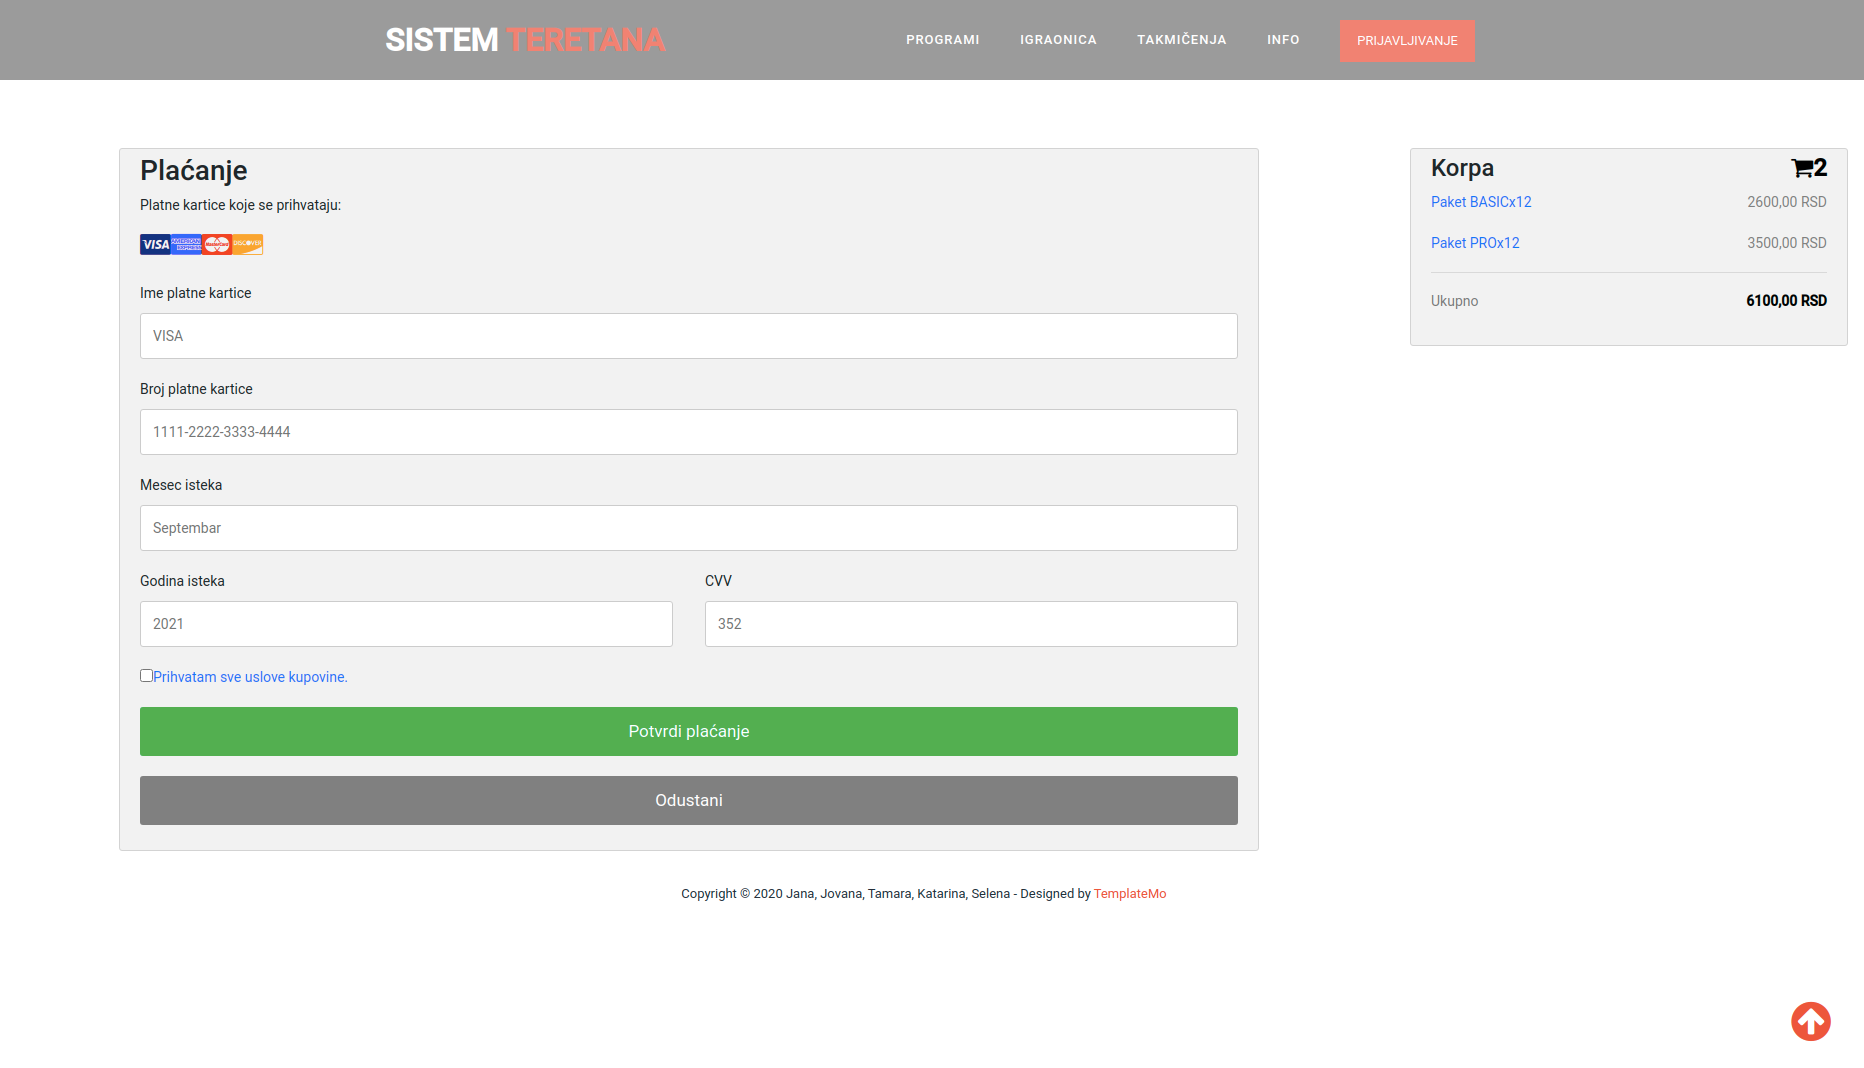
\includegraphics[scale=0.22]{sections/korisnicki_interfejs/screenshots/forma_za_placanje.png}
\end{center}
\caption{Forma za plaćanje}
\label{fig:forma}
\end{figure}

\end{document}
